\speaker{\Sergi{}}
\subsection{} % PAs besoin de titre

\begin{frame}
\frametitle{Conduire le projet}
Étapes mises en \oe{}uvre :
	\begin{itemize}
		\item Planifier
		\item Réaliser le suivi
		\item Gérer les risques et les opportunités
	\end{itemize}
\end{frame}

\subsection{}

\begin{frame}
\frametitle{Planifier}
\begin{itemize}
	\item Fiches de rôle
	\item Diagramme de Gantt
\end{itemize}
\begin{figure}
\begin{center}
	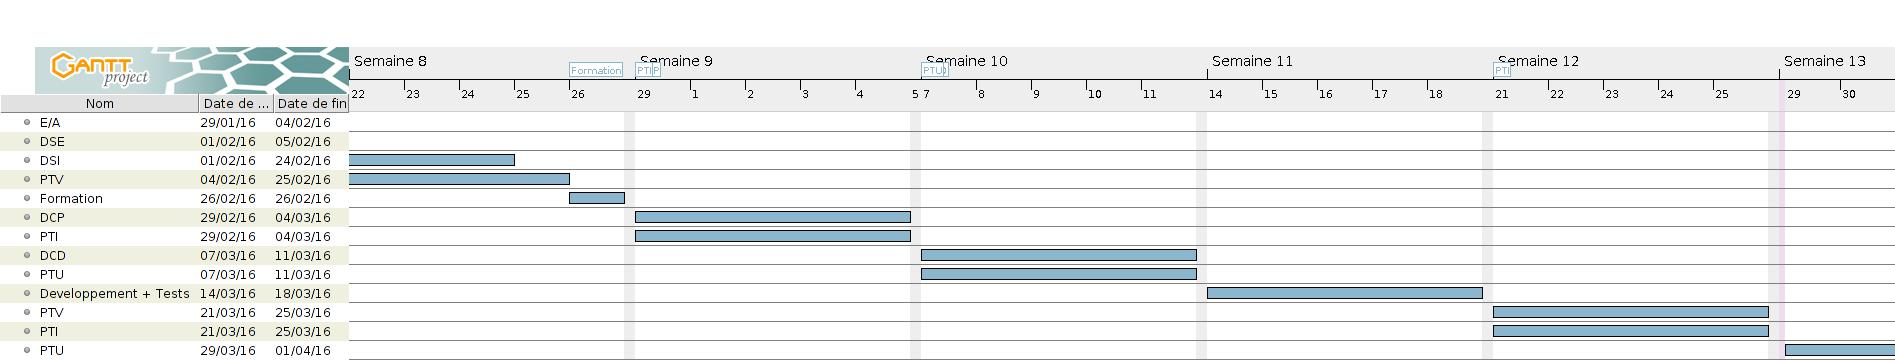
\includegraphics[scale=0.25]{images/exempleGantt.jpg}
	\caption{Diagramme de Gantt}
	\label{DG}
\end{center}
\end{figure}
\end{frame}

\begin{frame}
\frametitle{Planifier}
\begin{figure}
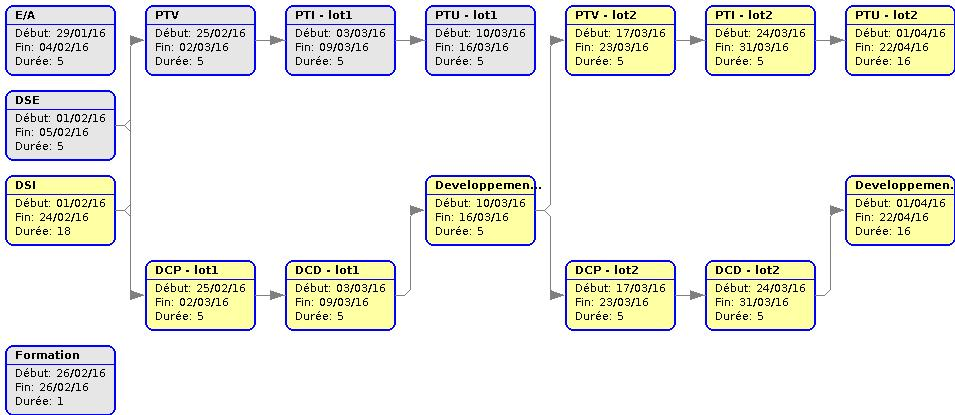
\includegraphics[scale=0.3]{images/exemplePert.jpg}
\caption{Diagramme de Pert}
\label{DP}
\end{figure}
\end{frame}

\subsection{}

\begin{frame}
\frametitle{Réaliser le suivi}
\begin{figure}
\begin{center}
\includegraphics[scale=0.4]{images/modeleSpirale.png}
\caption{Modèle en spirale}
\label{MS}
\end{center}
\end{figure}
\end{frame}

\begin{frame}
\frametitle{Kanban}
\begin{figure}
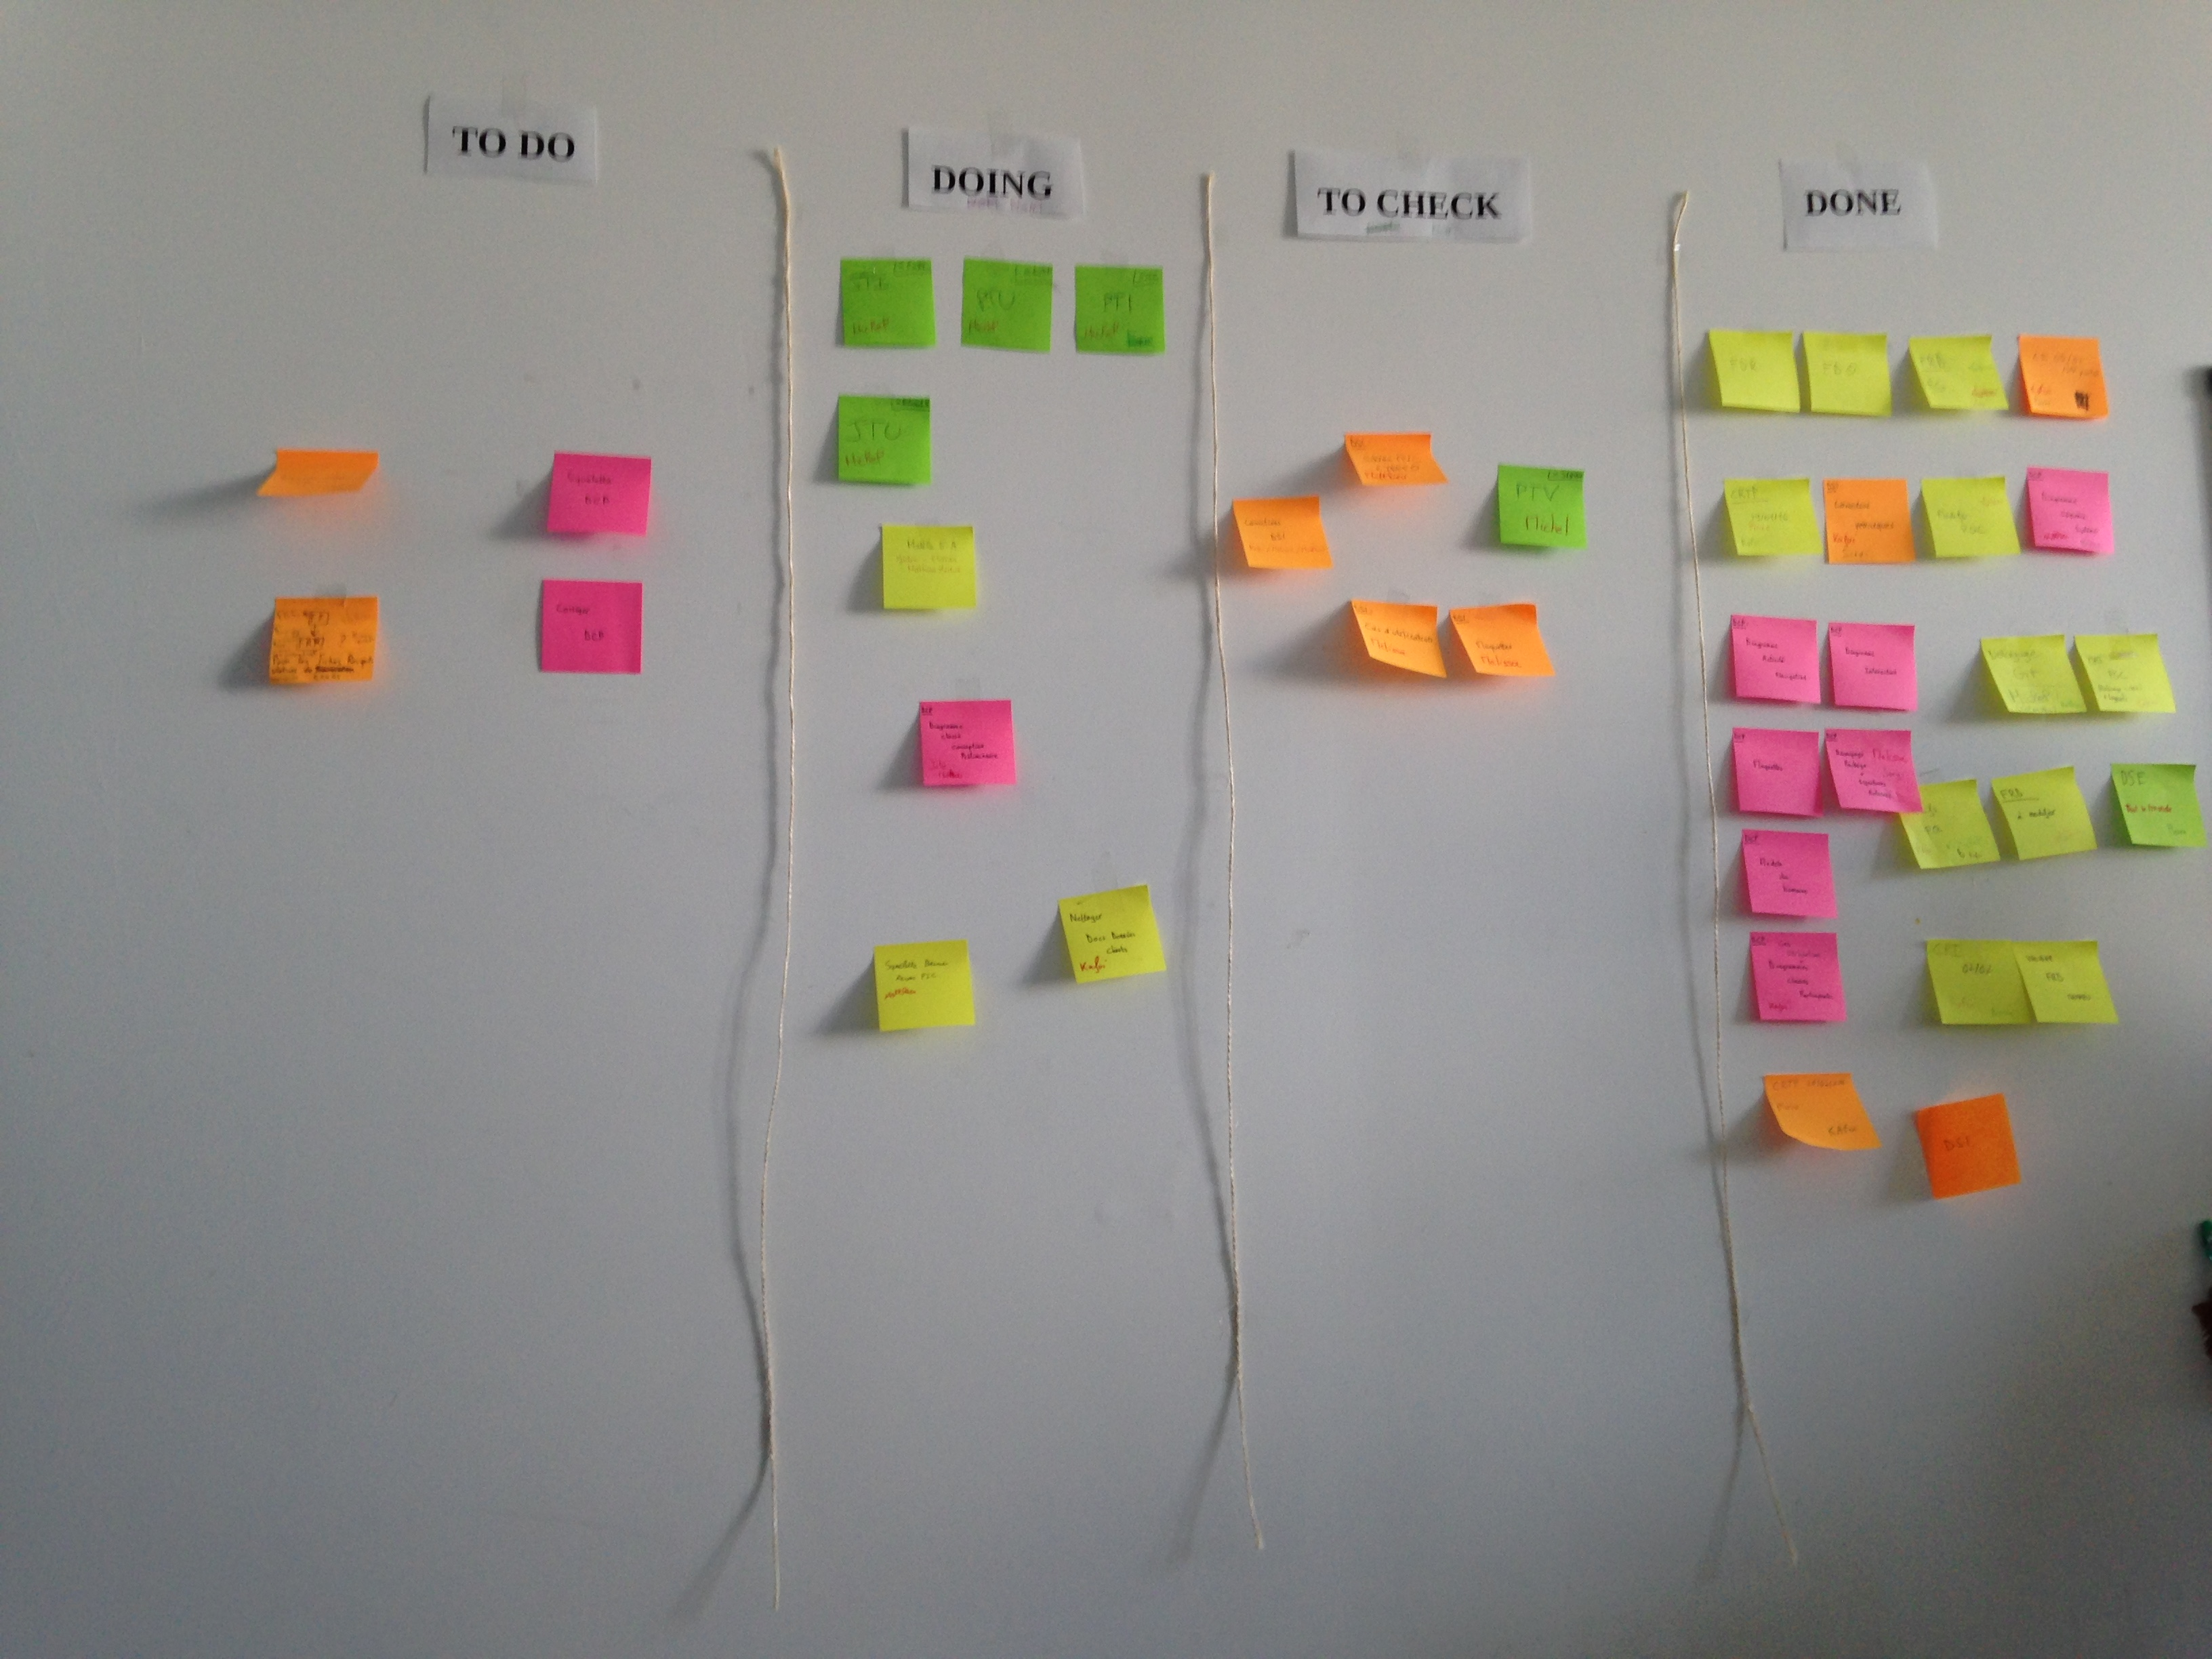
\includegraphics[scale=0.075]{images/kanban.JPG}
\caption{Kanban}
\label{Kn}
\end{figure}
\end{frame}

\begin{frame}
\frametitle{Procédures de communication}
Différentes procédures de communication :
\begin{itemize}
\item Communication interne
\item Communication inter PIC
\item Communication tuteurs
\item Communication client
\end{itemize}
\end{frame}
